\documentclass[a4paper,UTF8]{ctexart}

\usepackage{amsmath, amsthm, amssymb, amsfonts, hyperref, mathrsfs}%美国数学学会的包+?
\usepackage{geometry} %控制界面
\usepackage{bookmark}
\usepackage{fancyhdr} % header & footer
\usepackage{appendix} % 附录
\usepackage{tikz} %作图
\usepackage{graphicx} %插入图片的宏包
\usepackage{float} %设置图片浮动位置的宏包
%\usepackage{subfigure} %插入多图时用子图显示的宏包
\usepackage{listings} %引用代码
\usepackage{physics,mathtools} %物理数学工具
\usepackage{comment}
\usepackage{framed}
\usepackage{caption}
\usepackage{subcaption}
\geometry{top=2.5cm,bottom=2.5cm,left=2.5cm,right=2.5cm} % 布局要求
\pagestyle{fancy} % fancy分格
\fancyhf{} % 清除所有页眉页脚
\renewcommand\headrulewidth{0.6pt}
\renewcommand\footrulewidth{0.6pt}
% font
\setCJKmainfont{Noto Serif CJK SC}[BoldFont={Noto Serif CJK SC Bold}, ItalicFont=]
\lhead{何金铭 PB21020660$\mid$座位号:6}
\chead{磁光效应系列测量实验预习报告}
\rhead{\thepage}
\lfoot{2024.4.11}
\rfoot{USTC}
%\bibliographystyle{plain} % 引用样式
\everymath{\displaystyle} % display
%============================================================

\begin{document}

\begin{center}
    \textbf{\Large 磁光效应系列测量实验预习报告}
    \par \text{\large 何金铭 PB21020660}
\end{center}

\section{实验简介}

在外加磁场的作用下,物质的光学性质会发生改变,这就是磁光效应。
磁光效应主要包含磁光克尔效应、法拉第磁致旋光效应、科顿-穆顿磁致双折射效应。
在本实验中我们利用一套可以进行自由组合的实验装置,
通过搭建不同的测量光路来实现对这三种完全不同的磁光效应的测量。

\section{实验原理}

\subsection{磁光克尔效应}

当一束线偏振光入射到样品表面时, 反射光将变成椭圆偏振光且制偏光的长轴与入射光的偏振方向会发生偏转,
 如果样品处于铁磁状态, 铁磁性还会导致一个额外的偏转角度, 这个小角度称为克尔转角,
  记为 $\theta_{\mathrm{k}}$ 。而铁磁性也会导致椭偏率有一个附加的变化, 
  这个变化称为克尔粗偏率, 记为 $\varepsilon_{\mathrm{k}}$ 。
  由于 $\theta_{\mathrm{k}}$ 近似正比于样品的磁化强度 $M$ 的大小, 
  所以可以通过测量 $\theta_{\mathrm{k}}$ 得到磁化强度的信息。
  而测量 $\theta_{\mathrm{k}}$ 与外加磁场 $B$ 的关系, 
  可以反应出样品的磁化强度 $M$与外加磁场 $B$ 的关系, 近似得到样品的磁滞回线。

\begin{figure}[H]
    \centering
    \begin{minipage}[b]{0.9\textwidth}
        \centering
        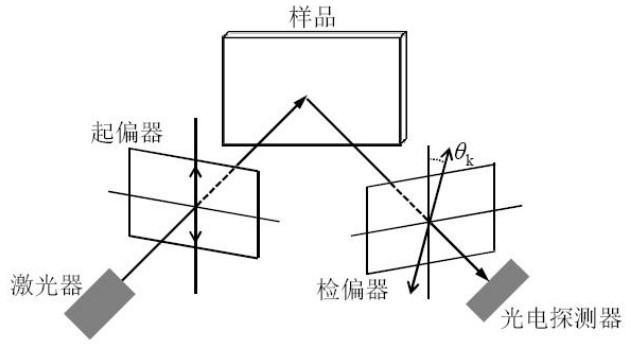
\includegraphics[width=0.9\textwidth]{./fig4.jpg}
        \caption{极向克尔效应测量原理图}
    \end{minipage}
\end{figure}

当外加磁场方向垂直于样品表面且平行于入射面时, 称为极向克尔效应, 
其测量原理如上图所示。为了简化实验, 选取入射光为电场矢量 $E_{\mathrm{s}}$ 
垂直于入射面的线偏振光。在样品处于未被磁化的初始状态时, 
反射光仍然是电场矢量垂直于入射面的线偏振光。当加上外加磁场后, 样品被磁化, 
由于极向克尔效应, 反射光中将含有一个很小的垂直于 $E_{\mathrm{s}}$ 的电场矢量
 $E_{\mathrm{p}}$ 。通常, 在一阶近似下有 
 $E_{\mathrm{p}} / E_{\mathrm{s}}=\theta_{\mathrm{k}}+\mathrm{i} \varepsilon_{\mathrm{k}}$ 。
 在本实验中, 设定检偏器的透光方向与 $E_{\mathrm{p}}$ 方向的
 夹角 $\delta$ 为 1 度左右, 此时通过检偏器的光强为:

\begin{equation}
I=\left|E_s \sin \delta+E_p \cos \delta\right|^2=\left|E_s\right|^2\left|\sin \delta+\left(\theta_k+i \varepsilon_k\right) \cos \delta\right|^2
\end{equation}

带入假设$\delta \ll 1, \theta_k,\varepsilon \ll \delta$可得极向克尔旋转角$\theta_k$为:

\begin{equation}
\theta_k=\frac{\delta}{2} \frac{I-I_0}{I_0}
\end{equation}

一般测量磁滞回线中正向饱和时的极向克尔旋转角 $\theta_k^{+}$和反向饱和时的极向克尔旋转角 $\theta_k^{-}$, 取其平均为该样品的极向克尔旋转角。

\begin{equation}
\theta_k=\frac{1}{2}\left(\theta_k^{+}-\theta_k^{-}\right)=\frac{\delta}{4} \frac{I\left(+M_s\right)-I\left(-M_s\right)}{I_0}=\frac{\delta}{4} \frac{\Delta I}{I_0}
\end{equation}

式中 $I\left(+M_{\mathrm{s}}\right)$ 和 $I\left(-M_{\mathrm{s}}\right)$ 分别是达到正负磁饱和状态下的反射光经检偏器的强度。

\subsection{法拉第磁致旋光效应}

在磁场的作用下,本来不具有旋光性的物质也产生了旋光性,即能使光矢量的振动面发生旋转,
这种现象称为法拉第效应或磁致旋光效应。法拉第效应中,
光振动方向的旋转角度$\theta_F$与光在介质中传播的距离$d$以及介质中的磁感应强度$B$成正比,即:

\begin{equation}
    \theta_F = V  B  d
\end{equation}

式中,$V$是表征物质磁光特性的系数,取决于样品介质的材料特性和光的波长,也称为费尔德(Verdet)系数。

\begin{figure}[H]
    \centering
    \begin{minipage}[b]{0.9\textwidth}
        \centering
        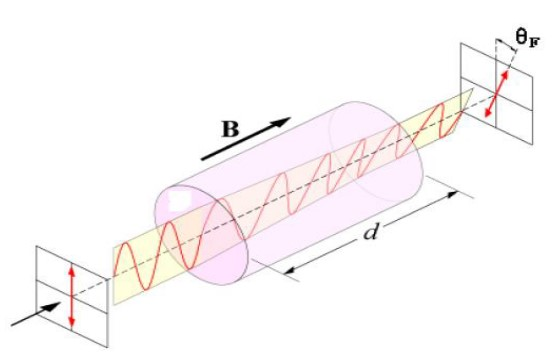
\includegraphics[width=0.9\textwidth]{./fig5.jpg}
        \caption{法拉第效应示意图}
    \end{minipage}
\end{figure}

采用与测量极向克尔旋转角相类似的方法, 也可以测量出法拉第效应中光振动方向的偏转角度
 $\theta_{\mathrm{F}}$, 进而求得样品的费尔德系数 $V$ 。在未加磁场的情况下,
  如果将检偏格兰棱镜偏离消光位置一个小角度 $\varphi$, 此时通过检偏后的透射光强 $I$ 可以表示为

\begin{equation}
    I = I_0 \sin^2{\varphi}
\end{equation}

式中 $I_0$ 为检偏格兰棱镜的入射光强。根据上式, 通过控制检偏角度 $\varphi$ 和测量透射光强 $I$,就可以求出 $I_0$, 从而避免直接测量 $I_0$ 。

加上一定的外加磁场后, 由于法拉第效应光的振动方向将旋转一定角度 $\theta_{\mathrm{F}}$, 此时通过检偏格兰棱镜后的透射光强 $I(B)$ 为

\begin{equation}
I(B)=I_0 \sin ^2\left(\varphi+\theta_F\right)
\end{equation}

通过测量透射光强 $I(B)$, 结合已知参数 $\varphi$ 和 $I_0$ 就可以求出法拉第旋转角 $\theta_{\mathrm{F}}$ 。

改变磁感应强度 $B$ 的大小, 进行一系列的测量, 就可得到 $\theta_{\mathrm{F}}$ 与 $B$ 的关系图。
知道样品的厚度后, 就可利用公式$\theta_F = V  B  d$求出材料的费尔德系数 $V$ 。

\subsection{磁致双折射效应}

磁流体是指磁性纳米颗粒在表面活性剂进行包覆或改性后,均匀分散到载液中,形成的胶体溶液。
当外加磁场时,磁流体中的磁性微粒会顺着磁场方向排列形成磁链,
使磁流体具有类似单轴晶体那样的双折射性质,这种现象称为科顿-穆顿效应。
磁场方向对应单轴晶体的“光轴”方向,入射光的传播方向与磁场方向垂直时,
o光的振动方向垂直于磁场方向,e光的振动方向平行于磁场方向。

实验证明,经过磁流体样品后o光与e光的相位差:

\begin{equation}
\Delta \varphi=\frac{2 \pi}{\lambda} \cdot d \cdot \Delta n=\frac{2 \pi}{\lambda} \cdot d \cdot\left(n_o-n_e\right)
\end{equation}

式中d是样品厚度。

\begin{figure}[H]
    \centering
    \begin{minipage}[b]{0.9\textwidth}
        \centering
        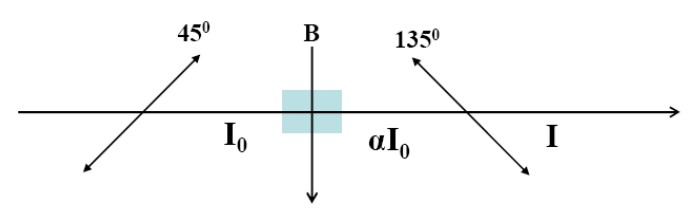
\includegraphics[width=0.9\textwidth]{./fig6.jpg}
        \caption{测量原理示意图}
    \end{minipage}
\end{figure}

本实验中,磁流体的透过率$\alpha$较小,不能近似为1,且o光和e光的强度透过率会随着磁场强度的大小变化,考虑到透过率的影响,检偏器的透射光强为:

\begin{equation}
I=\frac{1}{4} \cdot I_0 \cdot\left[\left(T_0+T_e\right)-2 \cos (\Delta \varphi) \sqrt{T_0 \cdot T_e}\right]
\end{equation}

式中 $T_0$ 和 $T_{\mathrm{e}}$ 分别为 $\mathrm{o}$ 光和 $\mathrm{e}$ 光的强度透过率,
 未加磁场时 $T_{\mathrm{o}}=T_{\mathrm{e}}=\alpha_{\circ}$ 加磁场后, 
 $T_{\mathrm{o}}$ 和 $T_{\mathrm{e}}$ 可分别写为 $T_0=\alpha k_0(\mathrm{~B}) 
 、 T_{\mathrm{e}}=\alpha k_{\mathrm{e}}(B)$, 其中 $k_0(B)$ 和 $k_{\mathrm{e}}(B)$
  为透过率的变化系数, $B=0$ 时, $k_0(B)=1$, $k_{\mathrm{e}}(B)=1$ 。上式可改写为:

\begin{equation}
I=\frac{1}{4} \cdot \alpha I_0 \cdot\left[\left(k_o+k_e\right)-2 \cos (\Delta \varphi) \sqrt{k_o \cdot k_e}\right]
\end{equation}

 由上式可知,为确定某磁场强度下 o 光与 e 光的相位差 Δφ及折射率差 $Δn (n_o-n_e)$, 需测量未加磁场时透过光强 $\alpha I_0$、在该磁场强度下通过检偏后的光强$I$ , 以及 o 光和 e 光的强度透过率变化系数$k_\mathrm{o}$和 $k_\mathrm{e\circ}$


\section{实验内容}

\subsection{测量镍薄膜的磁光克尔旋转角}

测量镍薄膜的磁光克尔旋转角。实验中需测量两种不同厚度(30 nm、50 nm) 
镍薄膜样品的“磁滞回线”(探测器输出电压与外加磁感应强度的关系),
 计算在磁化饱和时的克尔旋转角 $\theta_\mathrm{k}$, 并判断克尔转角的旋转方向。



\begin{figure}[H]
    \centering
    \begin{minipage}[b]{0.9\textwidth}
        \centering
        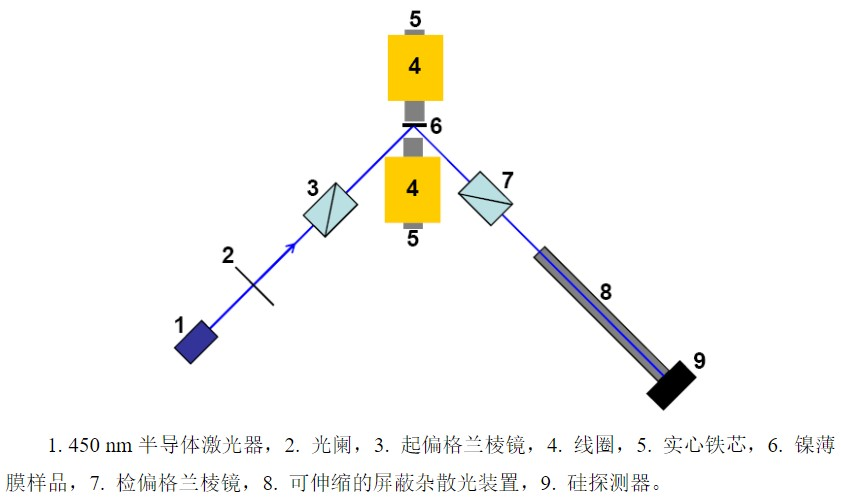
\includegraphics[width=0.9\textwidth]{./fig1.jpg}
        \caption{克尔效应测量光路示意图}
    \end{minipage}
\end{figure}

\subsection{测量蒸馏水的法拉第旋光系数}

测量蒸馏水的法拉第旋光系数。测量光程 $d$ 为 4 毫米的蒸馏水样品在不同磁场强度下, 法拉第旋转角 $\theta_\mathrm{F}$的大小,并判断旋转方向,计算出蒸馏水样品的费尔德系数 $\nu$。注:由于样品池为玻璃制品,也具有法拉第旋光效应,因此需先测出空样品池的旋转角,并在最后结果中扣除样品池的影响。



\begin{figure}[H]
    \centering
    \begin{minipage}[b]{0.9\textwidth}
        \centering
        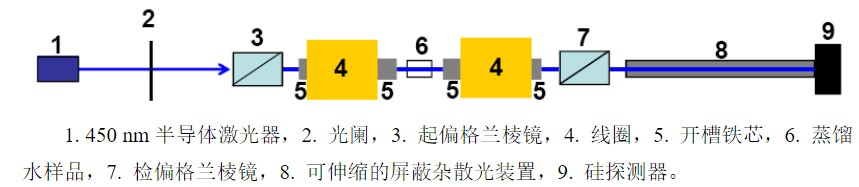
\includegraphics[width=0.9\textwidth]{./fig2.jpg}
        \caption{法拉第效应测量光路示意图}
    \end{minipage}
\end{figure}

\subsection{测量磁流体的磁致双折射(科顿-穆顿效应)的o光与e光的折射率差}

测量磁流体的磁致双折射(科顿-穆顿效应)的o光与 e 光的折射率差。

\begin{enumerate}
    \item 不加光阑
 和磁场时,观察入射线偏光的偏振方向与磁场垂直、平行和成 45°夹角三种情况下,
 通过磁流体样品后是否可以通过检偏格兰棱镜消光。在加磁场(励磁电流 1.5 A) 的条件下,
 再次观察上述三种情况。
    \item 测量不同磁场强度下,o 光和 e 光的强度透过率变化系数 
 $k_\mathrm{o}$ 和 $k_\mathrm{e}$, 检偏后的光强$I$,
 未加磁场时透过样品的光强 $\alpha I_0$,据此计算 o 光与 e 光的相位差 △φ及折射率差 $\Delta n$。
\end{enumerate}



\begin{figure}[H]
    \centering
    \begin{minipage}[b]{0.9\textwidth}
        \centering
        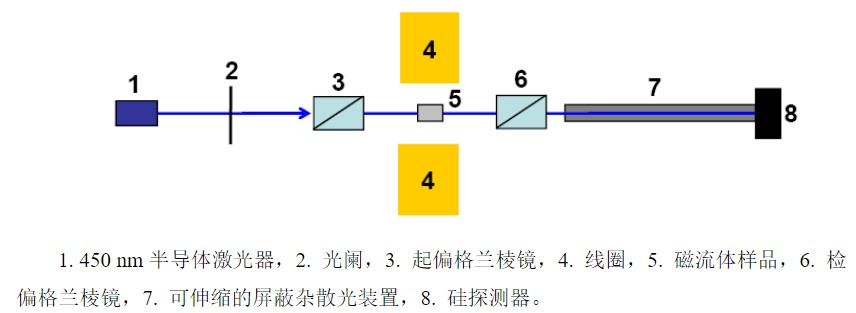
\includegraphics[width=0.9\textwidth]{./fig3.jpg}
        \caption{磁致双折射效应测量光路示意图}
    \end{minipage}
\end{figure}

\end{document}